\documentclass[12pt]{article}

\usepackage[a4paper, margin=2.5cm]{geometry}
\usepackage{graphicx}
\usepackage{rotating}
\usepackage[english]{babel}
\usepackage{appendix}
\usepackage{listings}
\usepackage{url}
\usepackage{todonotes}
\usepackage{tabularx}
\usepackage{amssymb}
\usepackage{tablefootnote}
\usepackage{appendix}

\graphicspath{{./resources}}
  
\title{COMP3900-H15A-capSquad - Project Proposal}
\date{\today}
\author{
    Daniel Latimer \\ z5115175 \and
    Connor O'Shea \\ z5115177 \and
    Kevin Chan \\ z5113136 \and
    Oliver Richards \\ z5157383 \and
    Peter Kerr \\ z5115807} 

\begin{document}

\maketitle
\tableofcontents
\newpage

\section{Background}
\subsection{Problem Domain}
With over 100 million monthly listeners\cite{musicoomph} and a steadily increasing user base, there is no doubt that podcasts are a greatly enriching source of information and entertainment for a large variety of individuals.

Although they are highly valuable, it can be difficult to find podcasts that are of interest to a particular user amidst the 1 million\cite{musicoomph} that are already available.
Thus, podcast streaming services (such as Ultracast) have been created, to provide a centralised place for exploring and discovering new podcasts that are valuable to the listener.

However, all of the web based podcast streaming services available lack many important features, and their interfaces leave much to be desired. For example, there is no streaming service that allows the user to bookmark certain parts of a podcast, nor take notes at certain timestamps. It is even difficult to find a service that allows the listener to change the playback speed of the podcast.

capSquad believes that there is no one service that combines all of the most important features together into a single package, leaving space in the market for a superior podcast streaming platform. We seek to fill this gap with our new web-based podcast streaming service, ultraCast.

\subsection{Existing Systems}
There are a number of existing podcast streaming services on the market. Some of the key failings that capSquad aims to rectify with ultraCast are listed in the following section, using Spotify\cite{spotify}, Sticher\cite{sticher} and Player FM\cite{player_fm} as case studies.
A summary of the comparison is shown in table \ref{table:podcast_comparison}.

All three solutions provide functionalities for users to listen and subscribe to podcasts.
Podcasts are recommended to users, however, the basis for these recommendations is not clear.

They also allow content creators to add podcasts to the respective platform.
In this regard Player FM is distinct from Spotify and Sticher, Player FM aggregates podcasts from iTunes or RSS feeds which are added by content creators or listeners. Player FM does not serve the podcasts itself.

As table \ref{table:podcast_comparison} shows, there are a number of key features that are not available on any platform. 
A podcast service which provides these features will improve the usability and engagement of the platform for listeners.

\begin{table}[ht]
    \centering
    \caption{Comparison of existing podcast services}
    \label{table:podcast_comparison}
    \bigskip
    \begin{tabularx}{\linewidth}{|X|c|c|c|}
    \hline
    \textbf{Feature} & \textbf{Spotify} & \textbf{Stitcher} & \textbf{Player FM} \\
    \hline
    Can see number of subscribers for podcasts & x & x & \checkmark \\
    \hline
    Finished episodes are marked as played & \checkmark & \checkmark & x \\
    \hline
    Notifications for new episodes added to subscribed podcasts & x & x & x \\
    \hline
    Centralised place to view previously listened to episodes & x & x & x \\
    \hline
    Recommended podcasts are stylized to the user & \checkmark & x & \checkmark \\
    \hline
    Can skip to previous episode & \checkmark & x & \checkmark \\
    \hline
    Can adjust playback speed & x & x & \checkmark \\
    \hline
    Closed captions & x & x & x \\
    \hline
    Ability to bookmark timestamps / take notes & x & x & x \\
    \hline
    Can follow other users & \checkmark & x & x \\
    \hline
    Can see the latest episode for each subscribed podcast in a preview panel & x & x & x \\
    \hline
    \end{tabularx}
\end{table}

\iffalse % Just commenting out this section(s)
\subsubsection{Spotify\cite{spotify}}

\todo{Do we want to keep the user stories here - I think its a bit confusing}

\begin{itemize}
    \item Cannot see number of subscribers for podcasts (UL-3)
    \item No notifications for new episodes added to subscribed podcasts (UL-9)
    \item No centralised place to view previously listened to episodes (UL-10, 11)
    \item Cannot adjust playback speed (UL-22)
    \item No closed captions (UL-25)
    \item No ability to bookmark timestamps, nor take notes (UL-26)
    \item Cannot see the latest episode for each subscribed podcast in a preview panel (UL-30)
\end{itemize}

\subsubsection{Sticher\cite{sticher}}

\begin{itemize}
    \item Cannot see number of subscribers for podcasts (UL-3)
    \item No notifications for new episodes added to subscribed podcasts (UL-9)
    \item No centralised place to view previously listened to episodes (UL-10, 11)
    \item Recommended podcasts are not stylized to the user (UL-13)
    \item Cannot skip to previous episode (only next) (UL-20)
    \item Cannot adjust playback speed (UL-22)
    \item No closed captions (UL-25)
    \item No ability to bookmark timestamps, nor take notes (UL-26)
    \item Cannot follow other users (UL-28)
    \item Cannot see the latest episode for each subscribed podcast in a preview panel (UL-30)
\end{itemize}

\subsubsection{Player FM\cite{player_fm}}
\begin{itemize}
    \item Finished episodes aren’t marked as played (UL-6)
    \item No notifications for new episodes added to subscribed podcasts (UL-9)
    \item No centralised place to view previously listened to episodes (UL-10, 11)
    \item No closed captions (UL-25)
    \item No ability to bookmark timestamps, nor take notes (UL-26)
    \item Cannot follow other users (UL-28)
    \item Cannot see the latest episode for each subscribed podcast in a preview panel (UL-30)
\end{itemize}

\fi


\newpage
\section{User Stories}

\subsection{Product Backlog}

The 29 user stories which make up the product backlog, as shown in Figure \ref{fig:backlog}, were grouped into three categories as described in the sections \ref{sec:project_objectives_stories}, \ref{sec:system_stories} and \ref{sec:novel_features_stories}.
Screenshots of the stories which make up the backlog can be found in sections \ref{sec:project_objectives_stories}, \ref{sec:system_stories} and \ref{sec:novel_features_stories}.

\begin{figure}[ht]
    \centering
    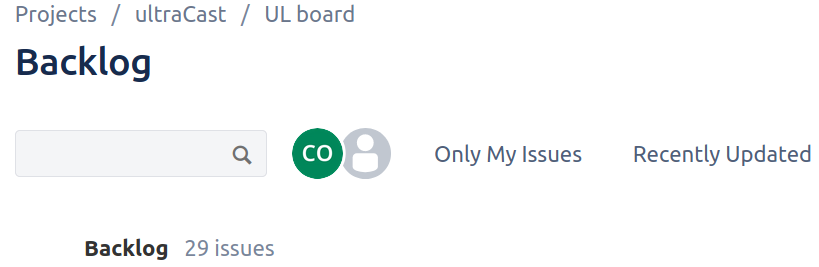
\includegraphics[width=10cm]{resources/project_backlog}
    \caption{ultraCast Backlog Count}
    \label{fig:backlog}
\end{figure}

\subsubsection{Project Objectives Stories} \label{sec:project_objectives_stories}

The project objective stories were derived directly from the project objectives. These JIRA stories can be found in Figure \ref{fig:jira_stories} below.
The mapping of each project objective to the final user story was summarised in Table \ref{table:project_objectives_to_stories}.

\begin{figure}[ht]
    \centering
    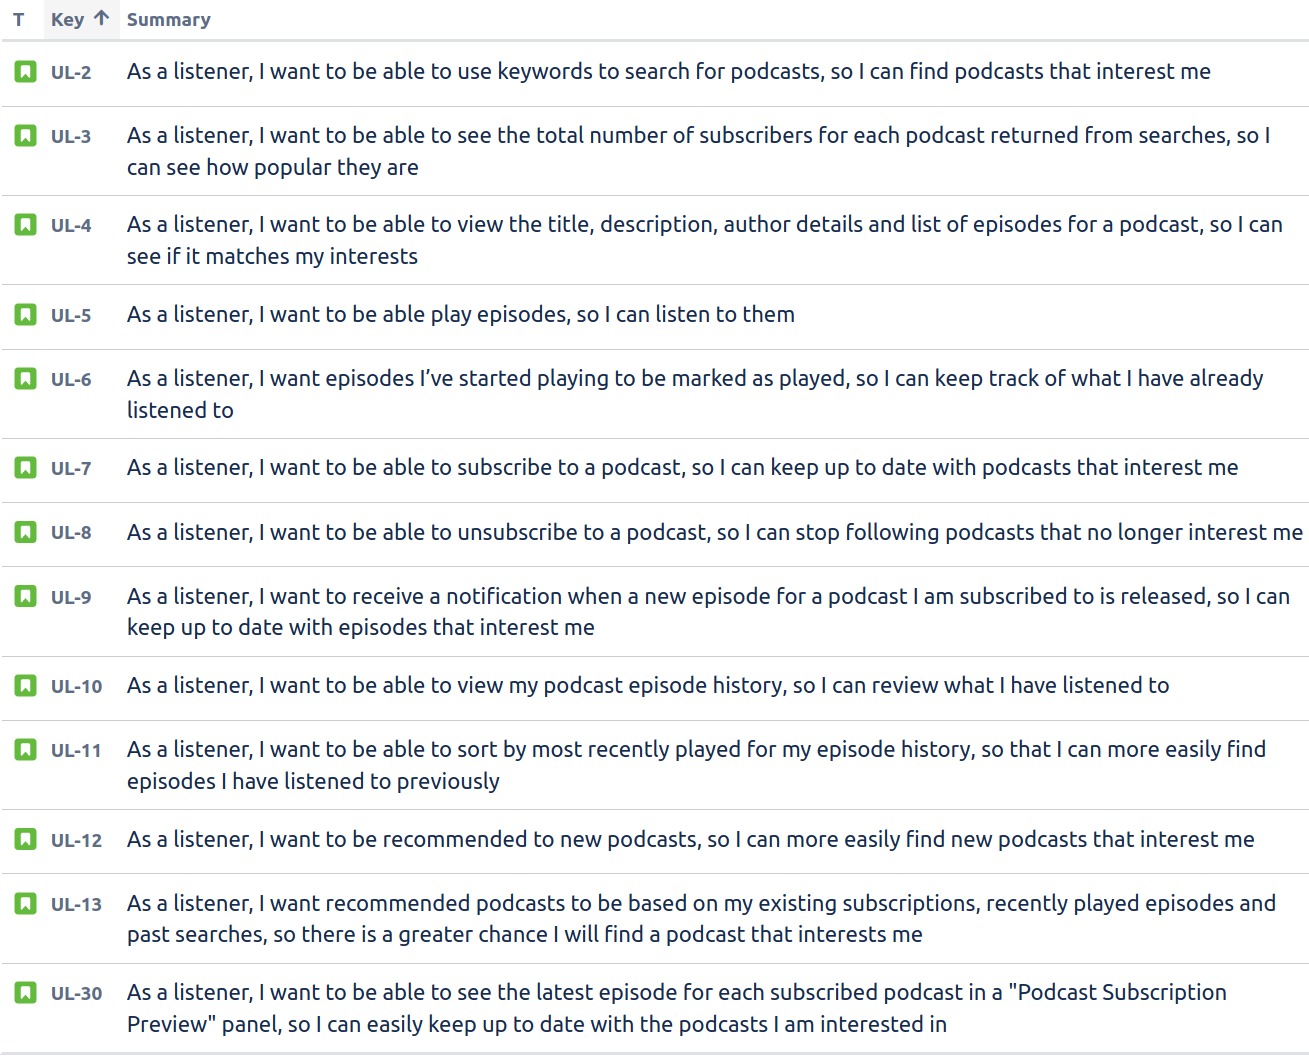
\includegraphics[width=\textwidth]{resources/objective_stories}
    \caption{JIRA Objective User Stories}
    \label{fig:jira_stories}
\end{figure}

\begin{table}
    \centering
    \caption{Project Objectives to Stories Mapping}
    \label{table:project_objectives_to_stories}
    \bigskip
    \begin{tabularx}{\linewidth}{|>{\hsize=1.8\hsize}X|>{\hsize=0.2\hsize}X|}
        \hline
        \textbf{Project Objective}                                             & \textbf{Story Key} \\
        \hline
        Listeners must be able to search for podcasts that interest them by keywords, resulting in a list of matching podcast titles, where the total number of subscriptions on the ultraCast platform (function described later) for each podcast is shown next to the title                                             & \begin{tabular}[c]{@{}l@{}}UL-2\\ UL-3\end{tabular}          \\ \hline
        Listeners must be able to select a podcast show from returned search results to view its full details, including its title, description, any author details that exist, as well as a list of episodes for the show                                             & UL-4                               \\ \hline
        Listeners must be able to play a selected episode within a podcast show, and once that episode starts being played, the listener must be able to also clearly see this episode marked as "Played"                                             & \begin{tabular}[c]{@{}l@{}}UL-5\\ UL-6\end{tabular}          \\ \hline
        Listeners must be able to subscribe or unsubscribe from a podcast show & \begin{tabular}[c]{@{}l@{}}UL-7\\ UL-8\end{tabular}         \\ \hline
        Listeners must be able to see the latest episode available for each show that they subscribed to in a "Podcast Subscription Preview" panel                                            & UL-30                              \\ \hline
        Listeners must be notified by the platform when a new episode for a show  they are subscribed appears                                             & UL-9                               \\ \hline
        Listeners must be able to see a history of the podcast episodes that they have played, sorted in order from most recently played to least recently played                                             & \begin{tabular}[c]{@{}l@{}}UL-10\\ UL-11\end{tabular}         \\ \hline
        ultraCast must be able to recommend new podcast shows to a listener based on at least information about the podcast shows they are subscribed to, podcast episodes they have recently played, and their past podcast searches                                             & \begin{tabular}[c]{@{}l@{}}UL-12\\ UL-13\end{tabular}         \\ \hline
    \end{tabularx}

    \iffalse
    \begin{tabular}{|l|l|}
        \hline
        \textbf{Project Objective}                                             & \textbf{\begin{tabular}[c]{@{}l@{}}Story\\ Key\end{tabular}} \\ \hline
        \begin{tabular}[c]{@{}l@{}}Listeners must be able to search for podcasts that interest them by keywords, \\ resulting in a list of matching podcast titles, where the total number of \\ subscriptions on the ultraCast platform (function described later) for each \\ podcast is shown next to the title\end{tabular}                                              & \begin{tabular}[c]{@{}l@{}}UL-2\\ UL-3\end{tabular}          \\ \hline
        \begin{tabular}[c]{@{}l@{}}Listeners must be able to select a podcast show from returned search results\\ to view its full details, including its title, description, any author details that \\ exist, as well as a list of episodes for the show\end{tabular}                                              & UL-4                               \\ \hline
        \begin{tabular}[c]{@{}l@{}}Listeners must be able to play a selected episode within a podcast show, and \\ once that episode starts being played, the listener must be able to also clearly \\ see this episode marked as "Played"\end{tabular}                                              & \begin{tabular}[c]{@{}l@{}}UL-5\\ UL-6\end{tabular}          \\ \hline
        Listeners must be able to subscribe or unsubscribe from a podcast show & \begin{tabular}[c]{@{}l@{}}UL-7\\ UL-8\end{tabular}         \\ \hline
        \begin{tabular}[c]{@{}l@{}}Listeners must be able to see the latest episode available for each show that \\ they subscribed to in a "Podcast Subscription Preview" panel\end{tabular}                                             & UL-30                              \\ \hline
        \begin{tabular}[c]{@{}l@{}}Listeners must be notified by the platform when a new episode for a show \\ they are subscribed appears\end{tabular}                                             & UL-9                               \\ \hline
        \begin{tabular}[c]{@{}l@{}}Listeners must be able to see a history of the podcast episodes that they have\\ played, sorted in order from most recently played to least recently played\end{tabular}                                             & \begin{tabular}[c]{@{}l@{}}UL-10\\ UL-11\end{tabular}         \\ \hline
        \begin{tabular}[c]{@{}l@{}}ultraCast must be able to recommend new podcast shows to a listener based \\ on at least information about the podcast shows they are subscribed to, \\ podcast episodes they have recently played, and their past podcast searches\end{tabular}                                             & \begin{tabular}[c]{@{}l@{}}UL-12\\ UL-13\end{tabular}         \\ \hline
    \end{tabular}
    \fi
    
\end{table}

\newpage
\subsubsection{System Stories} \label{sec:system_stories}

The system stories were designed to address common features offered by existing offerings in the same problem domain. 
They can be seen in Figure \ref{fig:jira_system_user_stories} below.

\begin{figure}[ht]
    \centering
    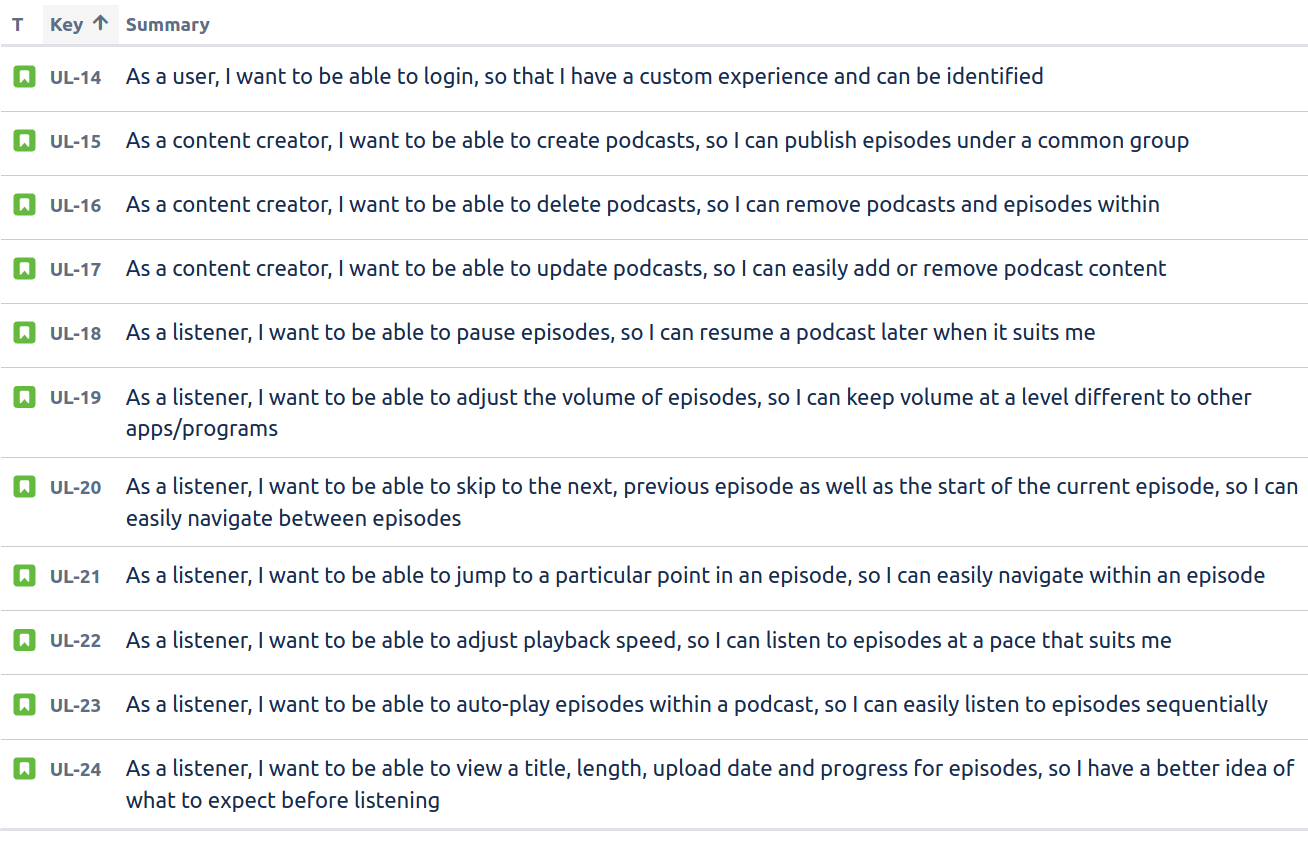
\includegraphics[width=\textwidth]{resources/system_stories}
    \caption{JIRA System User Stories}
    \label{fig:jira_system_user_stories}
\end{figure}

\newpage
\subsubsection{Novel Features Stories} \label{sec:novel_features_stories}

The novel feature user stories, as shown in Figure \ref{fig:jira_novel_user_stories}, were designed to create desirable features that are either uncommon or not 
available in other mainstream offerings in the same problem domain.

\begin{figure}[h]
    \centering
    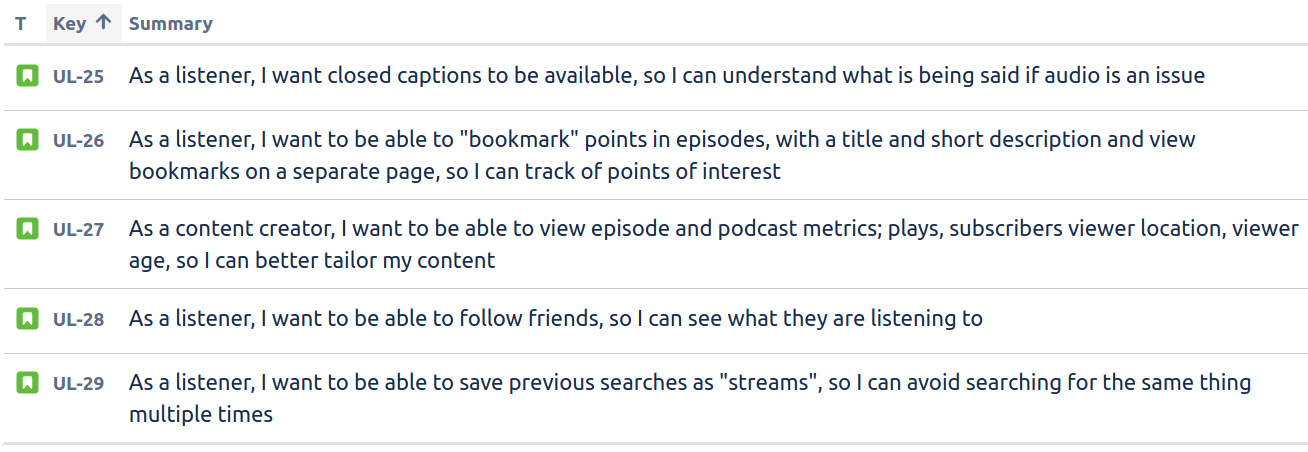
\includegraphics[width=\textwidth]{resources/novel_stories}
    \caption{JIRA Novel User Stories}
    \label{fig:jira_novel_user_stories}
\end{figure}

%\todo{format as table using competitiors and user story numbers in figure above}

\begin{table}[h]
    \centering
    \caption{Comparison of proposed novel features with competitiors. User stories are shown in figure \ref{fig:jira_novel_user_stories}}
    \label{table:comparison_features}
    \bigskip
    \begin{tabular}{|c|c|c|c|}
        \hline
        \textbf{User Story}      & \textbf{Spotify}      & \textbf{Stitcher}      & \textbf{Player FM} \\
        \hline
        UL-25           & X             & X             & X         \\
        \hline
        UL-26           & X             & X             & X         \\
        \hline
        UL-27           & \checkmark    & X             & X         \\
        \hline
        UL-28           & \checkmark    & X\tablefootnote{Some limited metrics on listening platform and number of view available}             & X         \\
        \hline
        UL-29           & X             & X             & X         \\
        \hline
    \end{tabular}
\end{table}

\subsection{Sprints}

The sprint planning will occur on Thursdays and the sprint duration will be exactly 
one week as seen in Table \ref{table:sprint_dates}.

\begin{table}
    \centering
    \caption{Sprint Dates}
    \label{table:sprint_dates}
    \bigskip
    \begin{tabular}{|l|l|l|}
    \hline
    \textbf{Week} & \textbf{Sprint Start} & \textbf{Sprint End} \\ \hline
    3-4           & 01/10/20              & 08/10/20            \\ \hline
    4-5           & 08/10/20              & 15/10/20            \\ \hline
    5-6           & 15/10/20              & 22/10/20            \\ \hline
    6-7           & 22/10/20              & 29/10/20            \\ \hline
    7-8           & 29/10/20              & 05/10/20            \\ \hline
    8-9           & 05/10/20              & 12/10/20            \\ \hline
    \end{tabular}
\end{table}

Relatively few stories were selected for the first sprint, as seen in Figure \ref{fig:first_sprint}
as there will be a decent amount of work in setting up the project infastructure. 
The sprints that were selected were those that focused on creating the data models 
(e.g. a podcast schema) which will be used later on by other stories, such as UL-2 
(search for podcasts).

\begin{figure}[ht]
    \centering
    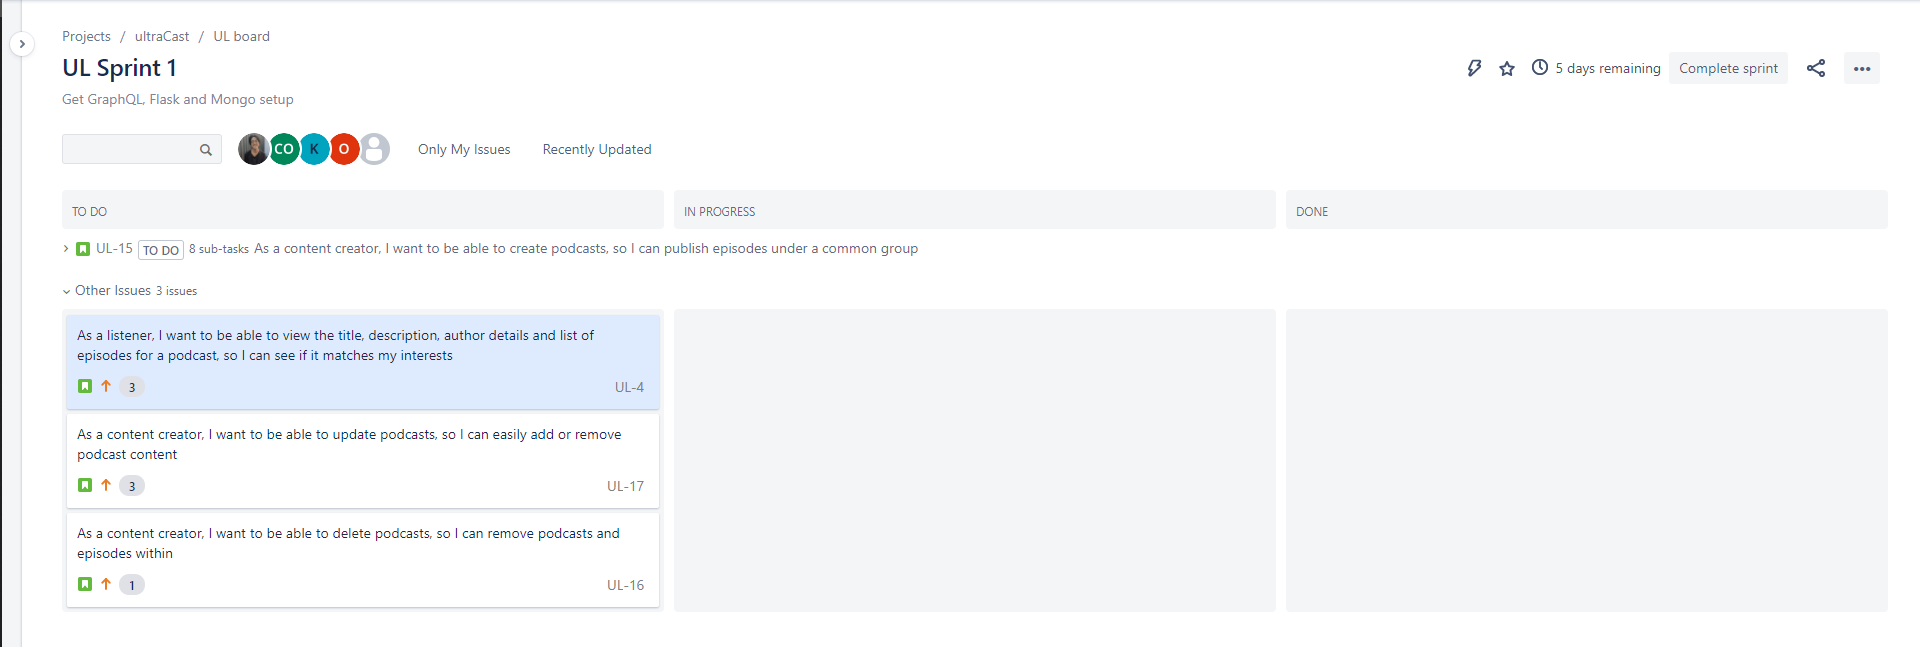
\includegraphics[width=\textwidth]{resources/sprint1}
    \caption{First Sprint (01/10/20 - 08/10/20)}
    \label{fig:first_sprint}
\end{figure}

\section{Interface and Flow Diagrams}

Identifying recommended podcasts for users involves a non-trivial backend implementation. Thus a flow diagram of the process is shown in figure \ref{fig:recommendation_engine_flowchart}.

Storyboards for all user stories are shown in appendix \ref{app:storyboards}.

\begin{figure}[h]
    \centering
    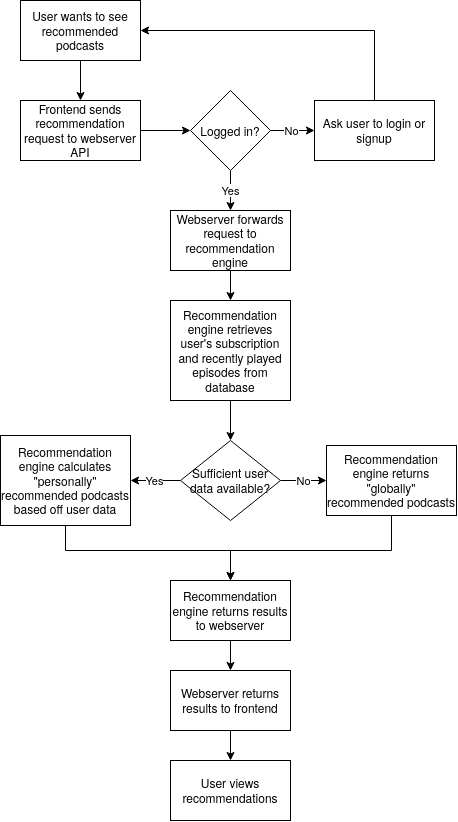
\includegraphics[height=0.5\paperheight]{resources/recommendation_engine}
    \caption{Flow Diagram of the recommendation process}
    \label{fig:recommendation_engine_flowchart}
\end{figure}

\section{System Architecture}

The proposed system architecture can be seen in Figure \ref{fig:SysArch}.
It can be seen that our end users will be podcast listeners and content creators.
First, we will use MongoDB\cite{MongoDB2020} to store our data, a NoSQL database that is popular for its high scalability.
This service will be interfaced with the MongoDB-Python driver, available on the MongoDB website\cite{MongoDB2020}.
Next, we will be using Flask\cite{flask} for our web-server: a micro-framework that allows us to quickly develop an MVP solution.
Flask is written in Python, so connecting to the database via the MongoDB-Python driver should be straightforward.
Additionally, we will have a recommendation service that will generate recommended podcasts based on the users listening history.
Finally, we will have a React\cite{react} frontend application that will enable our users to login, search and play podcasts, and get recommendations on ones they may be interested in.
The React application and Flask application will communicate through a GraphQL API: a scalable alternative to the popular REST API\cite{graphql}.

The architecture has been designed with the final demonstration in mind, hence, the business and presentation layers are shown to be hosted on the VLab machine.
Currently, MongoDB is not supported by Debian 6 (the Linux environment on the VLab machine), so we have opted to put the data layer onto an AWS EC2 instance\cite{aws_ec2}.

\begin{figure}[ht]
    \centering
    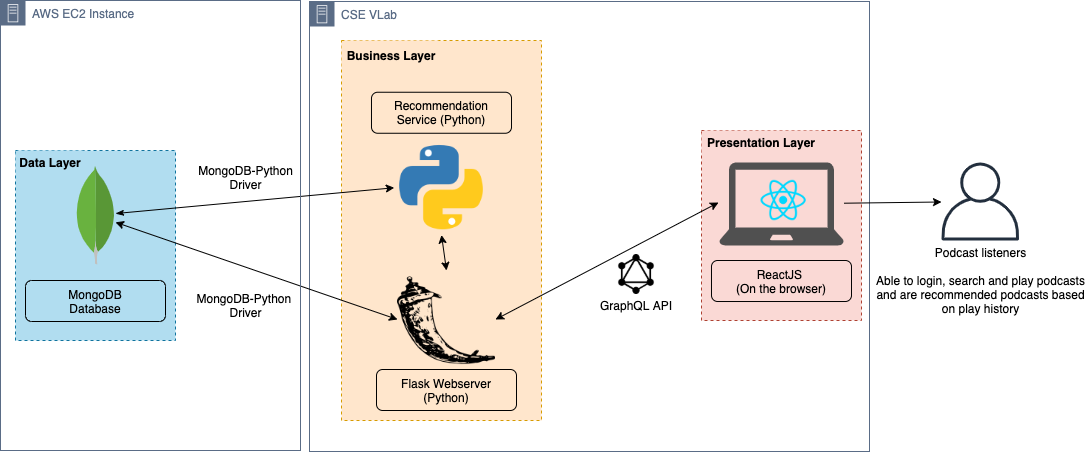
\includegraphics[width=\textwidth]{resources/SystemArchitecture}
    \caption{Proposed System Architecture}
    \label{fig:SysArch}
\end{figure}

\newpage
\bibliography{library.bib}
\bibliographystyle{plain}

\begin{appendices}
\section{Storyboards}\label{app:storyboards}
\begin{center}
    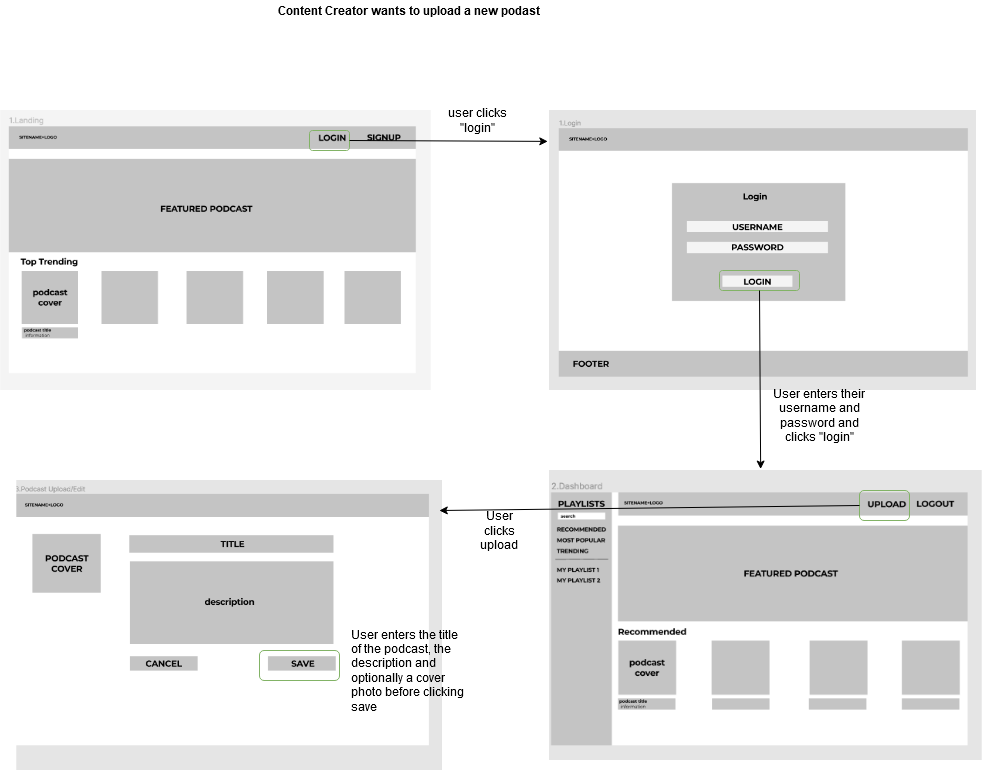
\includegraphics[width=\textwidth]{resources/uploading_podcasts}
    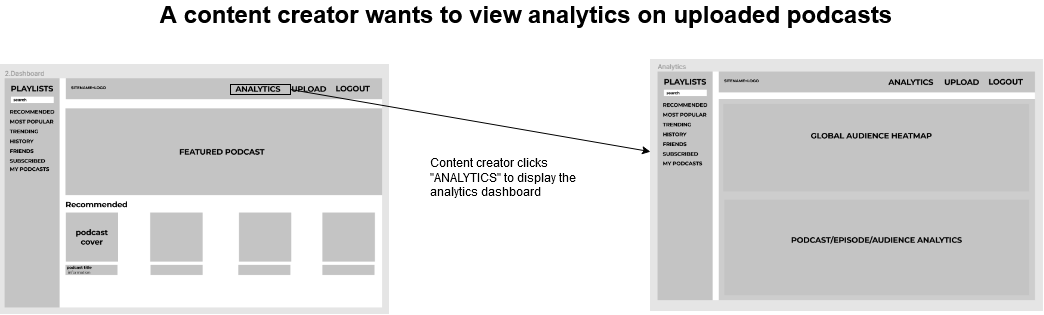
\includegraphics[width=\textwidth]{resources/analytics}
    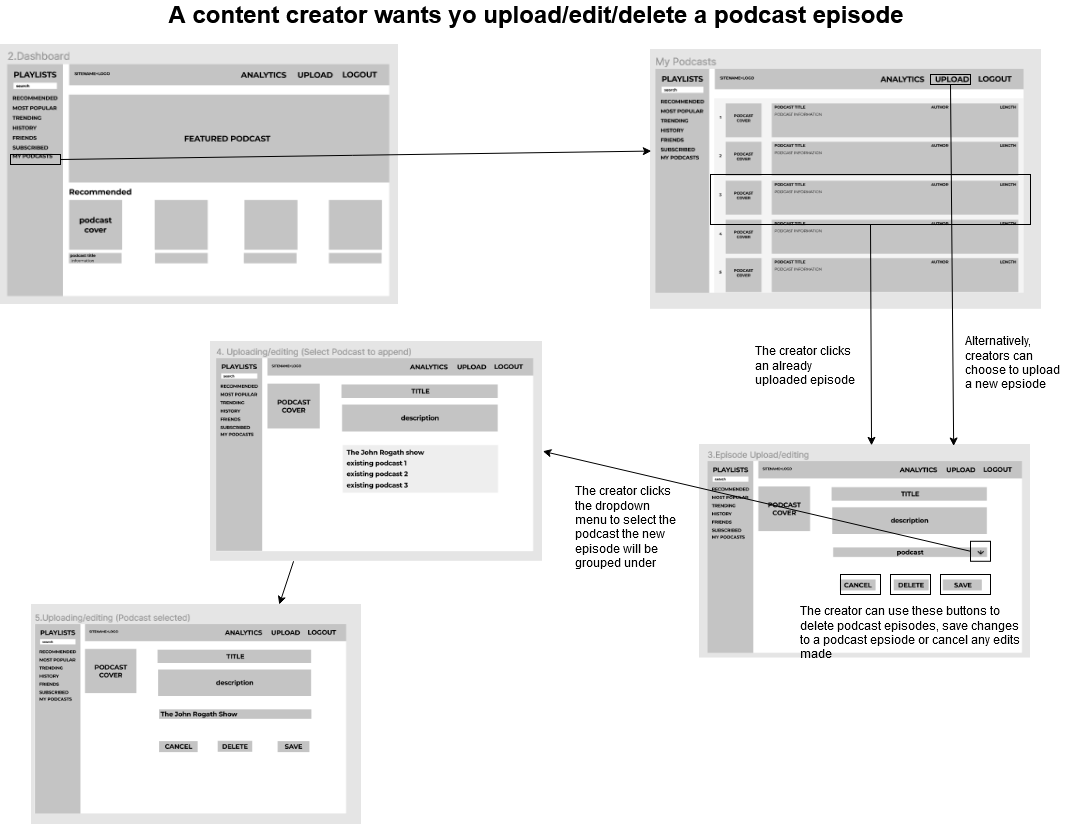
\includegraphics[width=\textwidth]{resources/upload_edit_delete}

    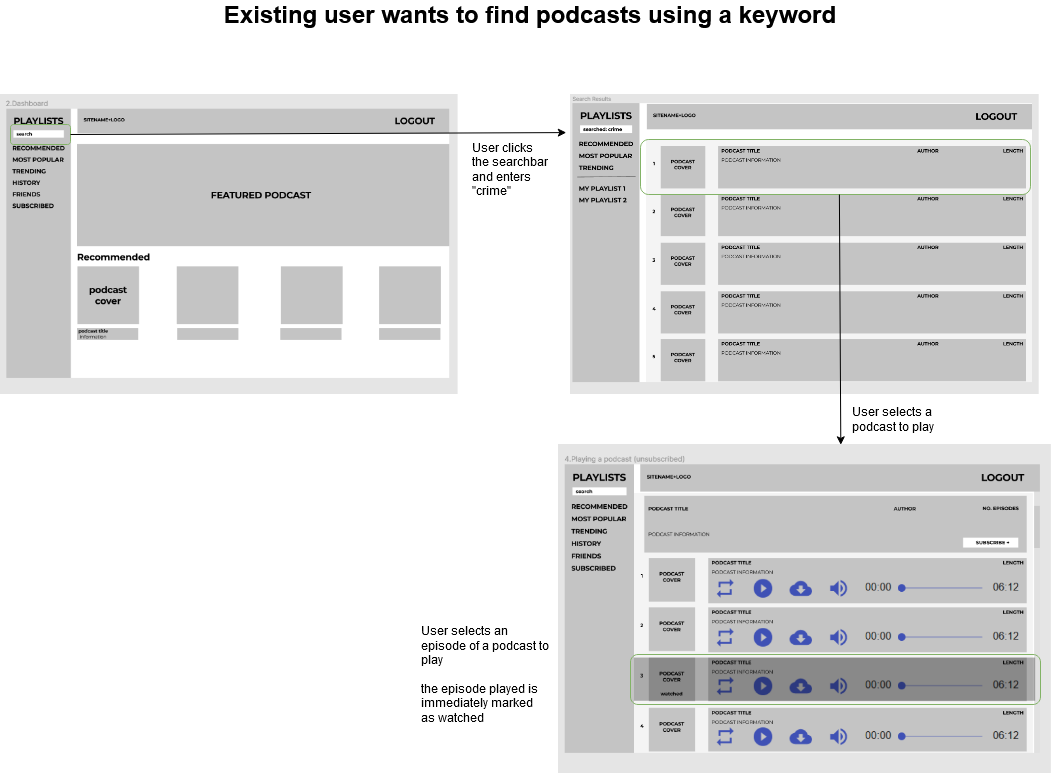
\includegraphics[width=\textwidth]{resources/search}
    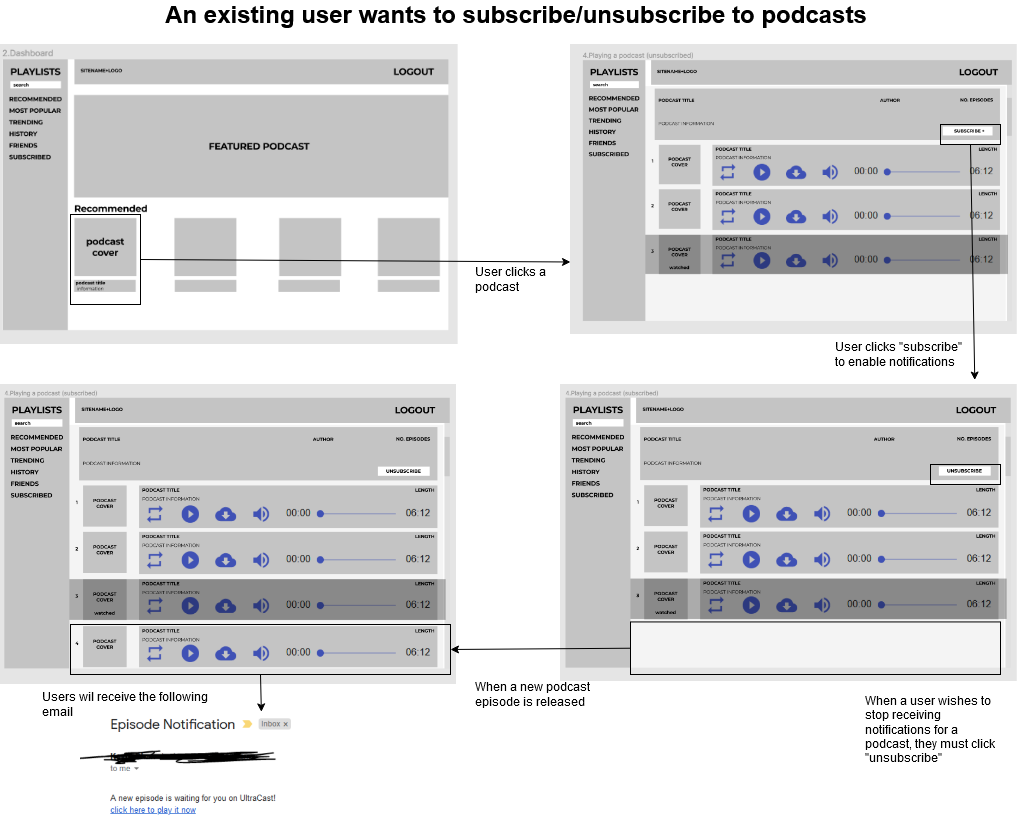
\includegraphics[width=\textwidth]{resources/subscribe}
    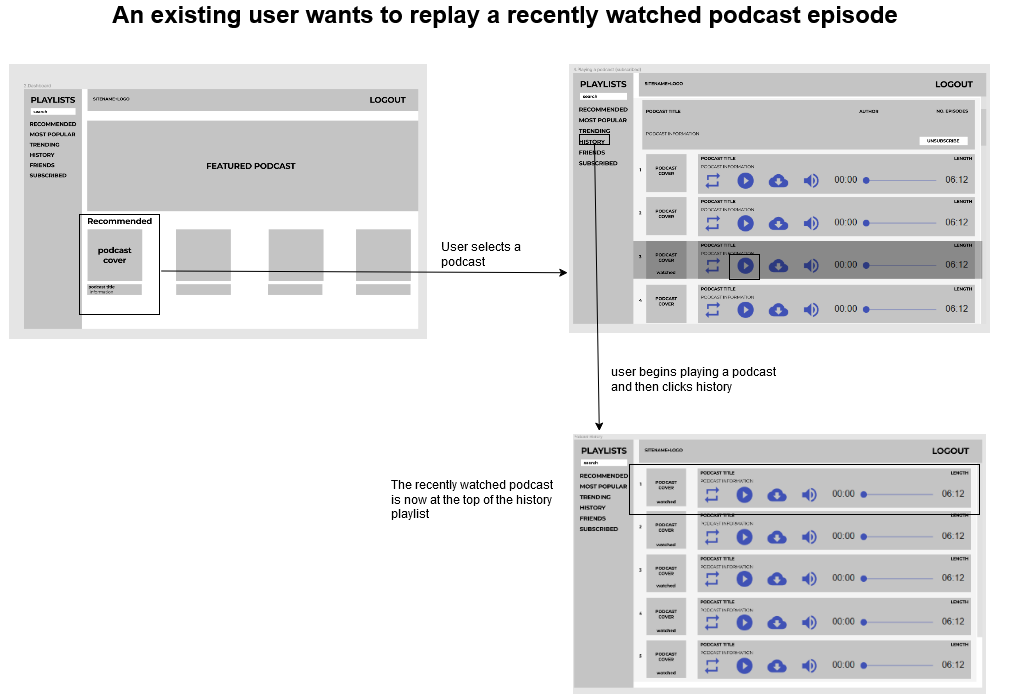
\includegraphics[width=\textwidth]{resources/history}
    \newpage
    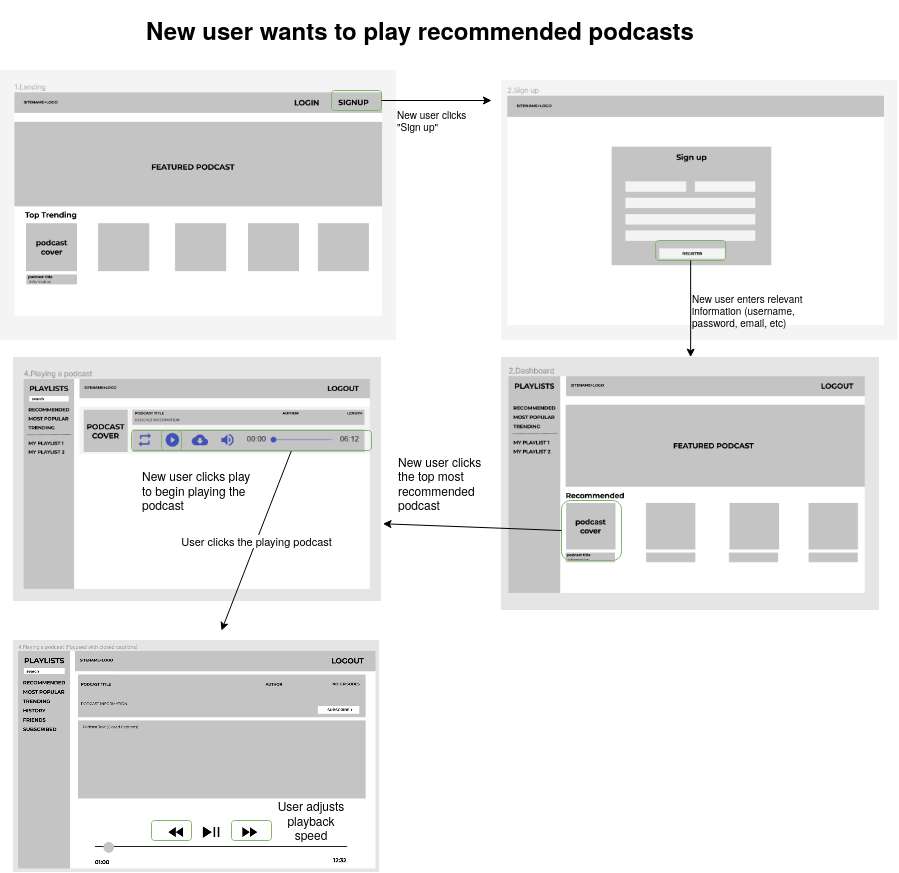
\includegraphics[width=\textwidth]{resources/playing_recommended_podcast_with_cc}
    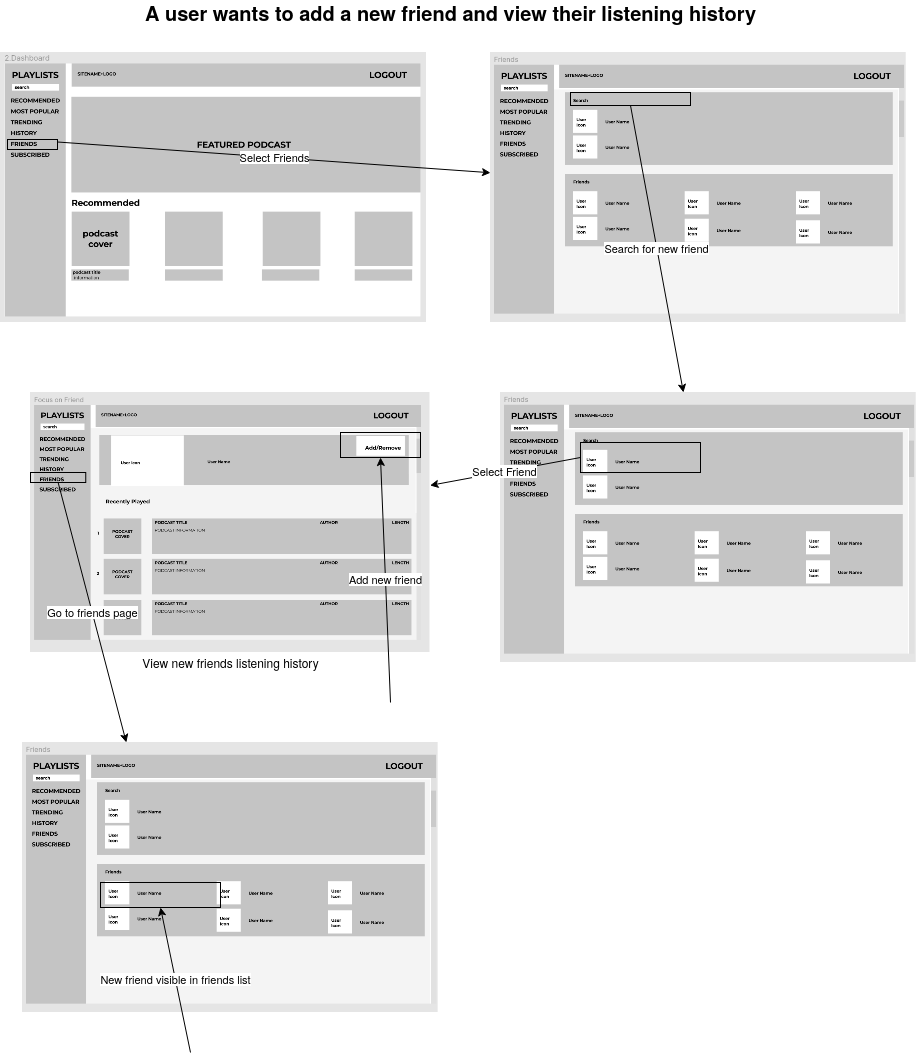
\includegraphics[width=\textwidth]{resources/friends}
    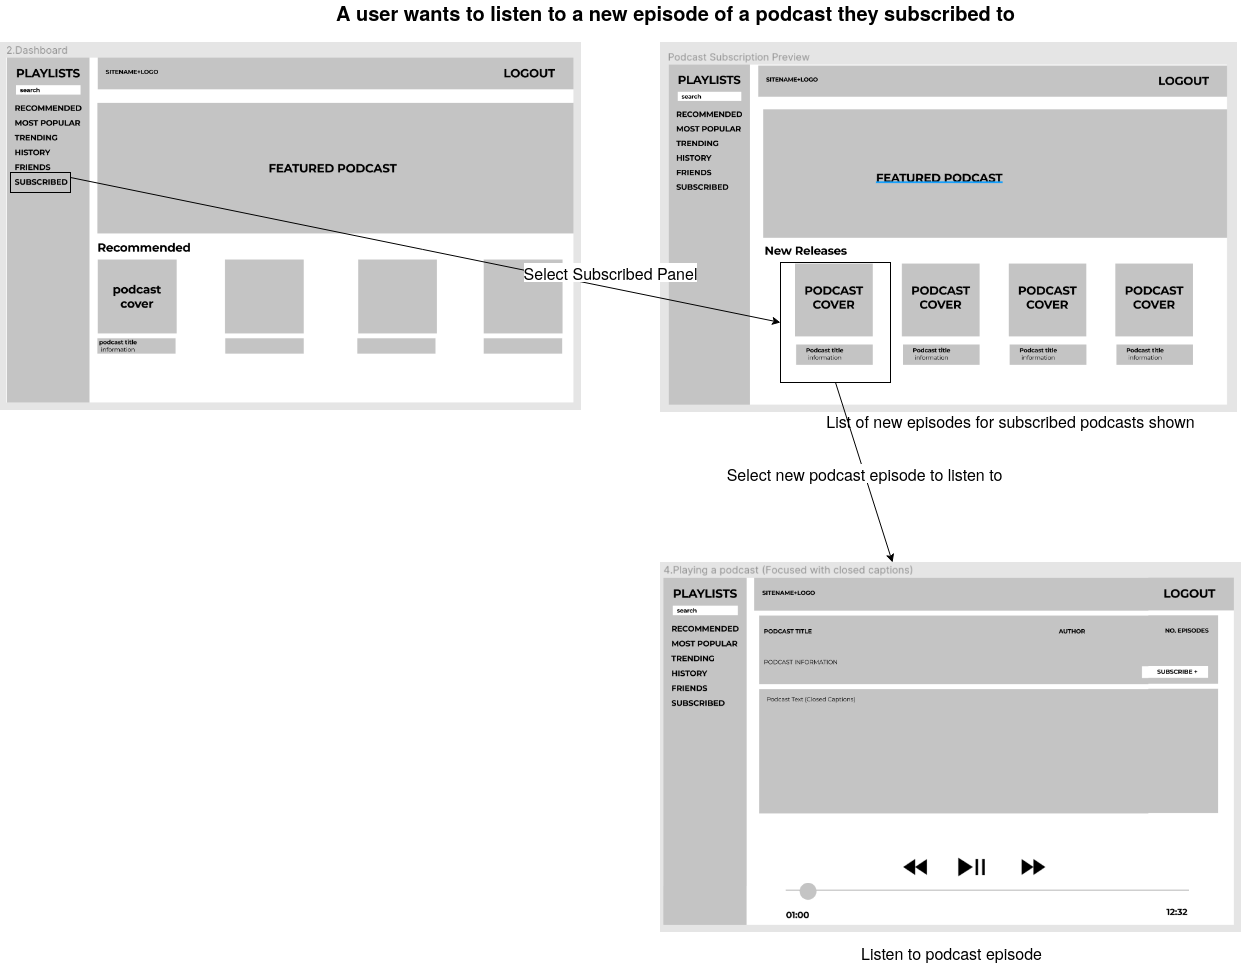
\includegraphics[width=\textwidth]{resources/podcast_subscription_preview}
    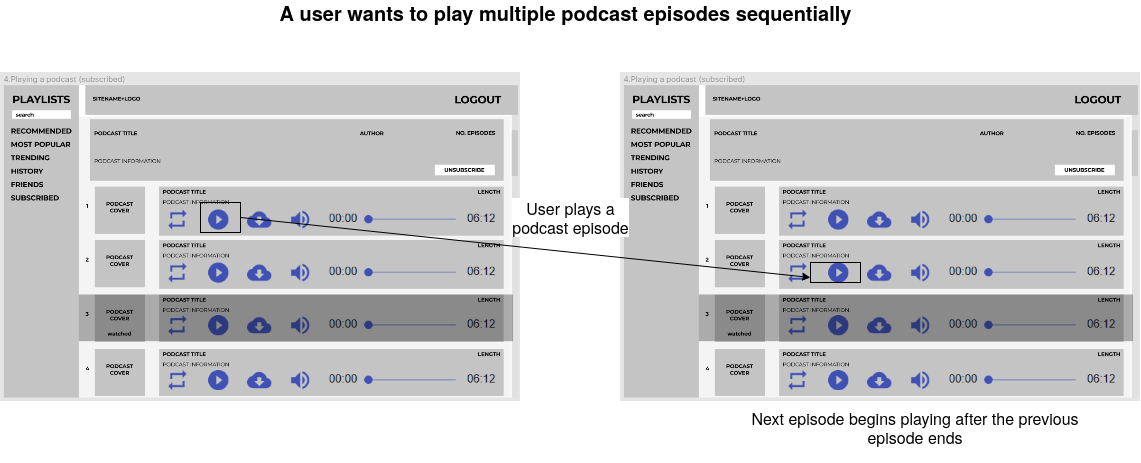
\includegraphics[width=\textwidth]{resources/autoplay}
    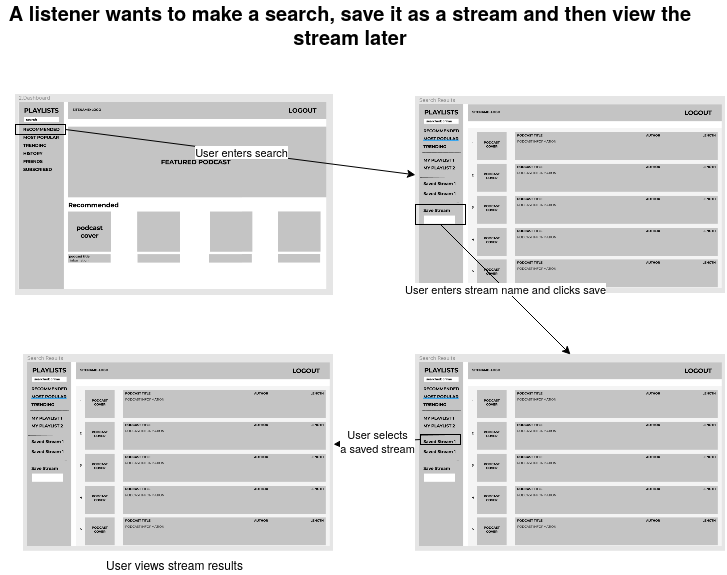
\includegraphics[width=\textwidth]{resources/save_stream}
\end{center}
\end{appendices}


\end{document}
